\documentclass[11pt]{article}
\usepackage{cs70_header}

\def\title{HW 2}

\begin{document}
\maketitle
\fontsize{12}{15}\selectfont

\begin{center}
    Due: Friday, 02/05  at 10:00 PM \\
    Grace period until Friday, 02/05 at 11:59PM
\end{center}

\section*{Sundry}

Before you start writing your final homework submission, state briefly how you worked on it. Who else did you work with? List names and email addresses. (In case of homework party, you can just describe the group.)

\Question{Stable Matching for Classes!}
%From sp14
Let's consider the system for getting into classes. For simplicity, we
will start with the problem assigning students to lab sections first,
since it is clear that there are a finite number of seats. We are given $n$
students and $m$ lab sections. 
Each lab section $\ell$ has some number, $q_\ell$ of seats, 
and we assume that the total number of students is larger than the total number of seats
(i.e. $\sum_{\ell=1}^m{q_{\ell}} < n$) and so some students are going to end
up with no lab. 
Each student ranks the $m$ lab sections in order of preference, and
the instructor for each lab ranks the $n$ students. 
Our goal is to find an assignment of students to seats (one student per seat) that is \textit{stable} 
in the following sense:
\begin{itemize}
\item There is no student-lab pair $(s,\ell)$ such that $s$ prefers $\ell$ to her allocated lab section
and the instructor for $\ell$ prefers $s$ to one of the students assigned to $\ell$. 
(This is like the stability criterion you have seen for jobs: 
it says there is no student-lab pair that would induce that lab instructor
to kick out an existing student and take this new student instead.)
\item There is no lab section $\ell$ for which the instructor prefers some unassigned student $s$ to one of the students assigned to $\ell$.
(This extends the stability criterion to take account of the fact that 
some students are not assigned to labs.)
\end{itemize}

Note that this problem is almost the same as the Stable Matching
problem for jobs/internships presented in the lecture note, with two differences:
(i) there are more students than seats; and
(ii) each lab section can have more than one seat.

Perhaps you will agree that this extended model is more realistic, even for the jobs context!

\begin{Parts}
\Part Explain how to modify the propose-and-reject algorithm so that 
it finds a stable assignment of students to seats.
[\textit{Hint}: What roles of students/instructors will be in the
propose-and-reject algorithm? What does ``candidates have a job offer
in hand (on a string)'' mean in this setting?]


\Part State a version of the Improvement Lemma (see the Stable
Matchings Lecture Note) 
that applies to your algorithm, and prove that it holds.

\Part Use your Improvement Lemma to give a proof that your algorithm terminates, that every seat is filled, and that the assignment your algorithm returns is stable.

\Part Let us consider the potential of a pair of students wishing to swap lab
sections, subject to global stability (i.e.~the swap can't make the
matching as a whole unstable). Either prove that your algorithm will
not have any such swap requests or modify it to have no such swap
requests and prove that the modified one will not have any pair of student
wanting to stably-swap sections.

\end{Parts}

\Question{Pairing Up}

Prove that for every even $n \geq 2$, there exists an instance of the stable matching problem with $n$ jobs and $n$ candidates such that the instance has at least $2^{n/2}$ distinct stable matchings.

\Question{A Better Stable Pairing}

In this problem we examine a simple way to {\em merge} two different
solutions to a stable matching problem. 
Let $R$, $R'$ be two distinct stable pairings.  Define the
new pairing $R \land R'$ as follows: 
\begin{quote}
For every job $j$, $j$'s partner in $R \land R'$ is whichever is better
(according to $j$'s preference list) of their partners in $R$ and $R'$.
\end{quote}
Also, we will say that a job/candidate \textit{prefers} a pairing $R$
to a pairing $R'$ if they prefers their partner in $R$
to their partner in $R'$. We will use the following example:

\begin{center}
\begin{tabular}{|c|c||c|c|}\hline
jobs&preferences& candidates & preferences \\
\hline
A& 1$>$2$>$3$>$4& 1 & D$>$C$>$B$>$A \\
\hline
B&2$>$1$>$4$>$3 & 2 & C$>$D$>$A$>$B  \\
\hline
C&3$>$4$>$1$>$2 & 3 & B$>$A$>$D$>$C  \\
\hline
D&4$>$3$>$2$>$1 & 4 & A$>$B$>$D$>$C  \\
\hline
\end{tabular}
\end{center}

\begin{Parts}
\Part $R=\{(A,4),(B,3),(C,1),(D,2)\}$ and
$R'=\{(A,3),(B,4),(C,2),(D,1)\}$ are stable pairings for the
example given above. Calculate $R \land R'$
and show that it is also stable.

\Part Prove that, for any pairings $R,\,R'$,
no job prefers $R$ or $R'$ to $R \land R'$.

\Part  Prove that, for any stable pairings $R,\,R'$
where $j$ and $c$ are partners in $R$ but not in $R'$, one of the following
holds:
\begin{quote}
$\bullet$ $j$ prefers $R$ to $R'$ and $c$ prefers $R'$ to $R$; or\\
$\bullet$ $j$ prefers $R'$ to $R$ and $c$ prefers $R$ to $R'$.
\end{quote}
[\textit{Hint}: Let $J$ and $C$ denote the sets of jobs and candidates respectively
that prefer $R$ to $R'$, and $J'$ and $C'$ the sets of jobs and candidates that prefer $R'$ to $R$.  Note that $|J|+|J'|=|C|+|C'|$. (Why is this?) Show that $|J| \leq |C'|$ and that $|J'| \leq |C|$.  Deduce that $|J'|=|C|$ and $|J|=|C'|$.  The claim should now follow quite easily.]

(You may assume this result in the next part even if you don't prove it here.)

\Part Prove an interesting result: for any stable pairings $R,\,R'$, (i) $R \land R'$ is a pairing [\textit{Hint}: use the results from (c)], and (ii) it is also stable.

\end{Parts}

\Question{Graph Basics}

In the first few parts, you will be answering questions on the following graph $G$.

\begin{figure}[h]
\centering
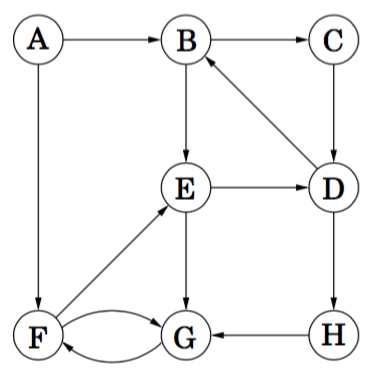
\includegraphics[width=5cm]{simple_graph.png}
\end{figure}

\begin{Parts}
\Part What are the vertex and edge sets $V$ and $E$ for graph $G$?

\Part  Which vertex has the highest in-degree? Which vertex has the lowest in-degree? Which vertices have the same in-degree and out-degree?

\Part  What are the paths from vertex $B$ to $F$, assuming no vertex is visited twice? Which one is the shortest path?

\Part  Which of the following are cycles in $G$?
\begin{enumerate}[i.]
\item $(B,C), (C,D), (D,B)$
\item $(F,G), (G,F)$
\item $(A,B), (B,C), (C,D), (D,B)$
\item $(B,C), (C,D), (D,H), (H,G), (G,F), (F,E), (E,D), (D,B)$
\end{enumerate}

\Part  Which of the following are walks in $G$?
\begin{enumerate}[i.]
\item $(E,G)$
\item $(E,G), (G,F)$
\item $(F,G), (G,F)$
\item $(A,B), (B,C), (C,D), (H, G)$
\item $(E,G), (G,F), (F,G), (G,C)$
\item $(E,D), (D,B), (B,E), (E,D), (D,H), (H,G), (G,F)$
\end{enumerate}

\Part  Which of the following are tours in $G$?
\begin{enumerate}[i.]
\item $(E,G)$
\item $(E,G), (G,F)$
\item $(F,G), (G,F)$
%\item $\{(A,B), (B,C), (C,D)\} $
%\item $\{(E,G), (G,F), (F,G), (G,F)\} $
\item $(E,D), (D,B), (B,E), (E,D), (D,H), (H,G), (G,F)$
\item $(B,C), (C,D), (D,H), (H,G), (G,F), (F,E), (E,D), (D,B)$
\end{enumerate}

\textbf{In the following three parts, let's consider a general undirected graph $G$ with $n$ vertices ($n \geq 3$).} If true, provide a short proof. If false, show a counterexample.

\Part  True/False: If each vertex of $G$ has degree at most 1, then $G$ does not have a cycle.

\Part  True/False: If each vertex of $G$ has degree at least 2, then $G$ has a cycle.

\Part  True/False: If each vertex of $G$ has degree at most 2, then G is not connected.

\end{Parts}

\Question{Proofs in Graphs} 

Please prove or disprove the following claims.

\begin{Parts}

\Part  On the axis from San Francisco traffic habits to Los Angeles traffic habits, Old California is more towards San Francisco: that is, civilized. In Old California, all roads were one way streets. Suppose Old California had 
$n$ cities ($n \geq 2$) such that for every pair of cities $X$ and $Y$,
either $X$ had a road to $Y$ or $Y$ had a road to $X$. Prove or disprove that
there existed a city which was reachable from every other city by traveling through at
most 2 roads. 

[\textit{Hint:} Induction]

\Part  
In lecture, we have shown that a connected undirected graph has an Eulerian tour if and only if every vertex has even degree.

Consider a connected graph $G$ with $n$ vertices which has exactly $2m$ vertices of
odd degree, where $m > 0$. Prove or disprove that there are $m$ walks that \emph{together} 
cover all the edges of $G$ (i.e., each edge of $G$ occurs in exactly one of the $m$ walks, 
and each of the walks should not contain any particular edge more than once).

\end{Parts}

\Question{Planarity}

\begin{Parts}
\Part Prove that $K_{3,3}$ is nonplanar.

\Part Consider graphs with the property $T$:
For every three distinct vertices $v_1, v_2, v_3$ of graph $G$, there are at
least two edges among them.
Use a proof by contradiction to show that if $G$ is a graph on $\ge 7$ vertices, and $G$ has property $T$, then
$G$ is nonplanar.

\end{Parts}

\end{document}